\chapter{Results}\label{sec:results}

This chapter presents the empirical findings from the analysis of 70 venture-backed software companies across 146 development periods during the \ac{ZIRP} era (2009-2022). The analysis reveals a context-dependent view of technical debt management that challenges conventional software engineering wisdom. The findings demonstrate that development velocity, rather than technical debt avoidance, serves as the primary predictor of funding success, with strategic debt accumulation potentially enhancing rather than constraining venture outcomes when paired with rapid execution.

\section{Sample Characteristics and Descriptive Analysis}\label{sec:sample_characteristics}

The final analytical dataset comprises 146 development periods from 70 venture-backed companies, representing a 95.4\% retention rate from the initial 153 potential development periods identified through systematic filtering. This high retention rate reflects the robust quality assurance applied to ensure analytical validity while maintaining sufficient sample size for meaningful statistical inference.

The filtering process, summarized in Table~\ref{tab:data_quality}, was designed to ensure that \ac{TDR} calculations reflect substantial software systems rather than early prototypes, and that development periods contain sufficient activity to generate meaningful velocity measurements. Of the 153 initial records, only 7 observations (4.6\%) were filtered due to insufficient data quality across multiple dimensions, with the primary exclusions arising from minimal development activity rather than fundamental data availability issues.

\begin{table}[htbp]
\centering
\caption{Data Quality Assessment and Filtering Results}
\label{tab:data_quality}
\begin{tabular}{lrr}
\hline
\textbf{Quality Criterion} & \textbf{Records} & \textbf{Retention Rate} \\
\hline
Initial development periods & 153 & 100.0\% \\
Valid TDR calculations (0 $\le$ TDR $\le$ 1) & 153 & 100.0\% \\
Sufficient codebase size (LOC > 5,000) & 151 & 98.7\% \\
Minimum period length (> 90 days) & 149 & 97.4\% \\
Minimum development activity (> 10 commits) & 146 & 95.4\% \\
\hline
\textbf{Final analytical sample} & \textbf{146} & \textbf{95.4\%} \\
\hline
\end{tabular}
\end{table}

The descriptive characteristics of the final sample, presented in Table~\ref{tab:descriptive_stats}, reveal the central tendencies of the key analytical variables. Development periods averaged 489 days, reflecting the diversity of funding cycles across different venture stages and market conditions. Technical debt ratios averaged 0.031, indicating that most companies in the sample maintained relatively modest levels of code-level debt. Development velocity averaged 0.089, with funding growth rates averaging 151.3\% between successive rounds.

\begin{table}[htbp]
\centering
\caption{Descriptive Statistics for Key Variables (N = 146 periods)}
\label{tab:descriptive_stats}
\begin{tabular}{lr}
\hline
\textbf{Variable} & \textbf{Mean} \\
\hline
Development period length (days) & 489.0 \\
Technical Debt Ratio & 0.031 \\
Development Velocity (composite) & 0.089 \\
Funding Growth Rate (\%) & 151.3 \\
\hline
\end{tabular}
\end{table}

Critically, the funding success rate across the sample is 54.1\%, meaning that slightly more than half of the development periods were followed by successful subsequent funding rounds. This balanced outcome distribution provides optimal conditions for analyzing the factors associated with venture capital success, avoiding the statistical challenges that would arise from heavily skewed success rates.

The sample comprises companies spanning six primary industry categories within the venture-backed software ecosystem, as detailed in Table~\ref{tab:industry_distribution_results}. The distribution reflects the broader venture ecosystem during the \ac{ZIRP} era, with infrastructure and developer-focused companies representing the largest segments. Notably, Database \& Storage companies achieved the highest funding success rate (64.3\%) while maintaining relatively high technical debt levels (0.083 average TDR) and high development velocity (0.161), exemplifying the Strategic Debt quadrant. Security companies also showed strong performance (66.7\% success rate) with the highest average technical debt levels (0.191 \ac{TDR}). Conversely, Business \& Application Software companies showed the lowest success rate (30.0\%) despite moderate debt levels. This variation across industries provides natural controls for examining whether debt-velocity relationships hold consistently across different market contexts and technical domains.

\begin{table}[htbp]
\centering
\caption{Industry Distribution and Performance Overview (N = 70 companies)}
\label{tab:industry_distribution_results}
\begin{tabular}{lrrrr}
\hline
\textbf{Industry Category} & \textbf{Companies} & \textbf{Success Rate} & \textbf{Avg TDR} & \textbf{Avg Velocity} \\
\hline
Developer Tools \& DevOps & 23 & 58.7\% & 0.043 & 0.113 \\
Database \& Storage & 18 & 64.3\% & 0.083 & 0.161 \\
Data Platform \& Analytics & 12 & 50.0\% & 0.049 & 0.127 \\
Business \& Application Software & 8 & 30.0\% & 0.063 & 0.108 \\
AI/Machine Learning & 4 & 42.9\% & 0.054 & 0.054 \\
Security & 5 & 66.7\% & 0.191 & 0.108 \\
\hline
\textbf{Total} & \textbf{70} & \textbf{54.1\%} & \textbf{0.031} & \textbf{0.089} \\
\hline
\end{tabular}
\end{table}

\section{Strategic Relationships: Debt, Velocity, and Funding Success}\label{sec:primary_relationships}

The analysis examines how technical debt and development velocity associate with funding outcomes, revealing unexpected patterns that challenge conventional assumptions. Understanding these relationships requires first establishing whether technical debt constrains development velocity as traditional engineering frameworks predict.

\subsection{The Debt-Velocity Relationship}

Examining the relationship between technical debt and development velocity, the company-level analysis reveals no significant relationship, though period-level patterns suggest potential complexity in this relationship. Table~\ref{tab:correlations} presents correlation results using both per-period and per-company approaches to address potential data dependency concerns. The per-period analysis shows a statistically significant positive correlation (r = 0.229, p = 0.005) between technical debt and development velocity, suggesting that higher debt levels associate with faster development rather than the anticipated velocity constraints. Critically, when analyzed at the company level (r = 0.056, p = 0.667), where data independence assumptions are satisfied, no significant relationship emerges.

Given the methodological requirement for independent observations, subsequent analyses and conclusions are based on the company-level results, while the period-level patterns provide supplementary descriptive context.

\begin{table}[htbp]
\centering
\caption{Correlation Analysis: Technical Debt, Velocity, and Funding Outcomes}
\label{tab:correlations}
\begin{tabular}{lrrl}
\hline
\textbf{Relationship} & \textbf{Correlation (r)} & \textbf{p-value} & \textbf{Significance} \\
\hline
\multicolumn{4}{l}{\textit{Per-period analysis (N = 146):}} \\
TDR $\leftrightarrow$ Development Velocity & 0.229 & 0.005 & Significant (p<0.01) \\
TDR $\leftrightarrow$ Funding Growth & 0.134 & 0.308 & Not Significant \\
Velocity $\leftrightarrow$ Funding Growth & -0.248 & 0.052 & Not Significant \\
\hline
\multicolumn{4}{l}{\textit{Per-company analysis (N = 70):}} \\
TDR $\leftrightarrow$ Development Velocity & 0.056 & 0.667 & Not Significant \\
\hline
\end{tabular}
\end{table}

With an R² of 0.052, technical debt explains only 5.2\% of the variance in development velocity, indicating that while statistically detectable, the practical relationship is weak. This finding suggests that technical debt accumulation may not impose the systematic velocity constraints assumed by traditional software engineering frameworks, at least within the range of debt levels observed in this venture-backed sample.

Turning to the relationship between development velocity and funding success, the analysis reveals additional complexity that requires examination through multiple lenses. Development velocity shows a negative correlation with funding growth rates (r = -0.248, p = 0.052), though this relationship is not statistically significant at conventional levels. This pattern potentially reflects different valuation dynamics, where high-velocity companies may achieve more frequent but smaller funding increments, while low-velocity companies must demonstrate exceptional market traction to justify continued investment.

However, when examining funding success as a binary outcome—the ability to secure subsequent rounds regardless of growth magnitude—development velocity emerges as a critical success factor. This distinction between funding probability and funding growth magnitude becomes central to understanding the strategic implications, as it suggests that velocity primarily influences investor confidence in continued viability rather than driving dramatic valuation increases.

The weak statistical relationship between technical debt and development velocity, combined with the complex relationship between velocity and funding outcomes, indicates that simple bivariate correlations may be insufficient for understanding strategic trade-offs in venture-backed environments. These findings motivate the strategic framework analysis that examines combined debt-velocity effects on funding success, potentially revealing interaction effects that are not apparent in individual correlation analyses.

\section{Strategic Framework and Robustness Analysis}\label{sec:strategic_framework_analysis}

To examine the combined effects of technical debt and development velocity on funding success, companies were classified into four strategic quadrants based on median splits of both variables. This framework reveals how different debt-velocity combinations associate with venture capital outcomes, providing insight into the strategic viability of debt accumulation when paired with rapid execution.

The strategic framework results, presented in Figure~\ref{fig:strategic_results_quadrants} and detailed in Table~\ref{tab:strategic_framework}, challenge conventional engineering wisdom by demonstrating that the Strategic Debt quadrant (high technical debt combined with high development velocity) achieves the highest funding success rate at 60.6\%. This finding suggests that strategic debt accumulation, when combined with high execution velocity, may actually enhance rather than constrain funding prospects in venture-backed environments.

\begin{figure}[htbp]
\centering
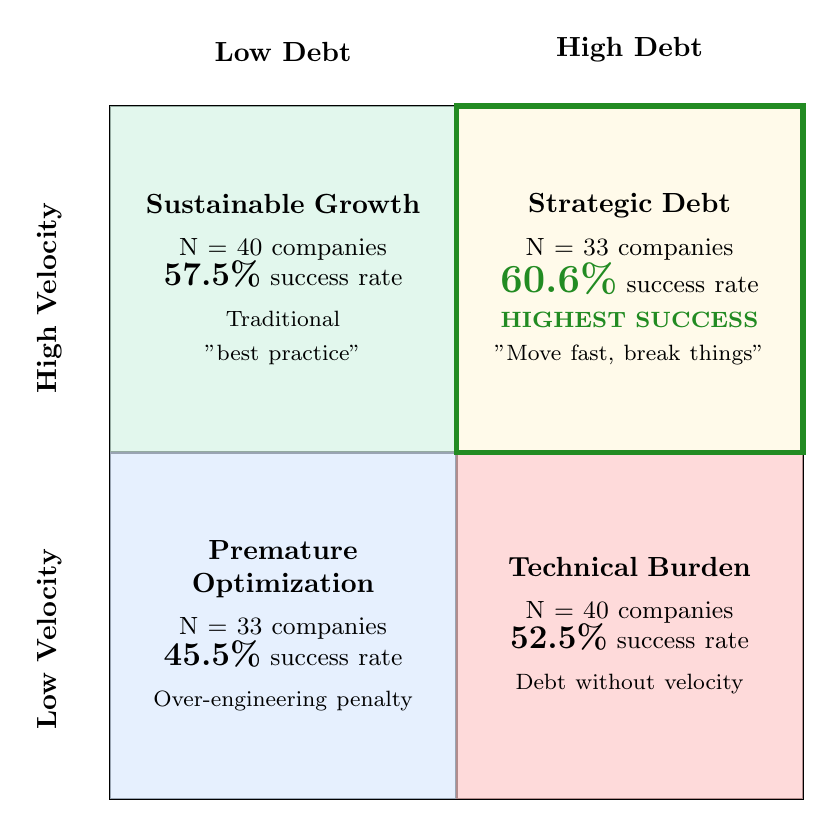
\begin{tikzpicture}[scale=1.1]
    % Define colors
    \definecolor{sustainable}{RGB}{213, 244, 230}
    \definecolor{strategic}{RGB}{255, 248, 225}
    \definecolor{premature}{RGB}{219, 234, 254}
    \definecolor{burden}{RGB}{254, 202, 202}
    \definecolor{winner}{RGB}{34, 139, 34}
    
    % Draw the main axes
    \draw[very thick] (-4,0) -- (4,0);
    \draw[very thick] (0,-4) -- (0,4);
    
    % Draw quadrant boxes
    \draw[thick] (-4,-4) rectangle (0,0);  % Bottom-left
    \draw[thick] (0,-4) rectangle (4,0);   % Bottom-right
    \draw[thick] (-4,0) rectangle (0,4);   % Top-left
    \draw[thick] (0,0) rectangle (4,4);    % Top-right
    
    % Fill quadrants with colors
    \fill[sustainable, opacity=0.7] (-4,0) rectangle (0,4);    % Top-left: Sustainable Growth
    \fill[strategic, opacity=0.7] (0,0) rectangle (4,4);     % Top-right: Strategic Debt
    \fill[premature, opacity=0.7] (-4,-4) rectangle (0,0);   % Bottom-left: Premature Optimization
    \fill[burden, opacity=0.7] (0,-4) rectangle (4,0);      % Bottom-right: Technical Burden
    
    % Highlight the winning quadrant with thick border
    \draw[winner, very thick, line width=2pt] (0,0) rectangle (4,4);
    
    % Axis labels
    \node[above] at (-2,4.4) {\textbf{Low Debt}};
    \node[above] at (2,4.4) {\textbf{High Debt}};
    
    \node[left, rotate=90] at (-4.7,3) {\textbf{High Velocity}};
    \node[left, rotate=90] at (-4.7,-1) {\textbf{Low Velocity}};
    
    % Quadrant content - Top-left (Sustainable Growth)
    \node[text width=3.5cm, align=center] at (-2,2) {
        \textbf{Sustainable Growth}\\[0.15cm]
        \small N = 40 companies\\
        \textbf{\large 57.5\%} \small success rate\\[0.1cm]
        \footnotesize Traditional "best practice"
    };
    
    % Quadrant content - Top-right (Strategic Debt) - WINNER
    \node[text width=3.5cm, align=center] at (2,2) {
        \textbf{Strategic Debt}\\[0.15cm]
        \small N = 33 companies\\
        \textcolor{winner}{\textbf{\Large 60.6\%}} \small success rate\\[0.05cm]
        \textcolor{winner}{\footnotesize \textbf{HIGHEST SUCCESS}}\\
        \footnotesize "Move fast, break things"
    };
    
    % Quadrant content - Bottom-left (Premature Optimization)
    \node[text width=3.5cm, align=center] at (-2,-2) {
        \textbf{Premature Optimization}\\[0.15cm]
        \small N = 33 companies\\
        \textbf{\large 45.5\%} \small success rate\\[0.1cm]
        \footnotesize Over-engineering penalty
    };
    
    % Quadrant content - Bottom-right (Technical Burden)
    \node[text width=3.5cm, align=center] at (2,-2) {
        \textbf{Technical Burden}\\[0.15cm]
        \small N = 40 companies\\
        \textbf{\large 52.5\%} \small success rate\\[0.1cm]
        \footnotesize Debt without velocity
    };
    
    % Add crown symbol for winner
    \node[winner, scale=1.5] at (3.6, 3.5) {$\bigstar$};
    
\end{tikzpicture}
\caption{Strategic Framework Results: Funding Success by Debt-Velocity Combinations (N=146 periods)}
\label{fig:strategic_results_quadrants}
\end{figure}

The Sustainable Growth quadrant (low debt + high velocity), representing traditional engineering best practices, achieves a 57.5\% success rate—lower than the Strategic Debt approach. This pattern suggests that pure debt avoidance may not be optimal when it constrains the rapid iteration and feature delivery that venture capital markets reward. The Premature Optimization quadrant shows the lowest success rate at 45.5\%, providing empirical evidence that over-engineering at the expense of velocity may be counterproductive in venture-backed environments where market timing and demonstrated momentum are critical.

\begin{table}[htbp]
\centering
\caption{Strategic Framework: Performance Metrics by Quadrant}
\label{tab:strategic_framework}
\begin{tabular}{lrrrrr}
\hline
\textbf{Strategic Quadrant} & \textbf{N} & \textbf{Success Rate} & \textbf{Avg TDR} & \textbf{Avg Velocity} & \textbf{Funding Growth} \\
\hline
\textbf{Sustainable Growth} & & & & & \\
(Low Debt + High Velocity) & 40 & 57.5\% & 0.014 & 0.185 & 144.5\% \\
\hline
\textbf{Strategic Debt} & & & & & \\
(High Debt + High Velocity) & 33 & 60.6\% & 0.133 & 0.229 & 161.7\% \\
\hline
\textbf{Premature Optimization} & & & & & \\
(Low Debt + Low Velocity) & 33 & 45.5\% & 0.013 & 0.048 & 141.4\% \\
\hline
\textbf{Technical Burden} & & & & & \\
(High Debt + Low Velocity) & 40 & 52.5\% & 0.091 & 0.046 & 272.6\% \\
\hline
\end{tabular}
\end{table}

Despite low success rates, companies in the Technical Burden quadrant achieve the highest average funding growth (272.6\%) when successful.
This suggests that while investors are initially skeptical of their technical capabilities, exceptional market traction can overcome these doubts. The subsequent large funding rounds then serve as both a catch-up investment and a premium for the high risk undertaken

Examining the patterns across quadrants reveals a consistent velocity effect. Table~\ref{tab:velocity_effect} isolates this by comparing success rates across debt levels while controlling for velocity differences. Among low-debt companies, high velocity provides a 12.0 percentage point advantage in funding success, while among high-debt companies, high velocity provides an 8.1 percentage point advantage. This consistent "velocity premium" suggests that rapid execution capability represents a fundamental competitive advantage in venture-backed environments, with debt levels playing a secondary moderating role.

\begin{table}[htbp]
\centering
\caption{Development Velocity Effect on Funding Success by Debt Level}
\label{tab:velocity_effect}
\begin{tabular}{lccc}
\hline
\textbf{Debt Level} & \textbf{Low Velocity} & \textbf{High Velocity} & \textbf{Velocity Premium} \\
\hline
Low Technical Debt  & 45.5\% & 57.5\% & +12.0 pp \\
High Technical Debt & 52.5\% & 60.6\% & +8.1 pp \\
\hline
\end{tabular}
\end{table}

\subsection{Robustness Testing Across Classification Schemes}

To test whether these findings are artifacts of the median-split methodology, the analysis was repeated using tertile (3×3) and quartile extreme (2×2) classification schemes. The tertile analysis, dividing each metric into low, medium, and high categories, reinforces the velocity-driven pattern while revealing additional nuances in optimal debt levels. The detailed tertile results are provided in Appendix~\ref{app:tertile_analysis}, but the key finding remains consistent: high-velocity development associates with superior funding outcomes across different debt levels.

Building on the tertile analysis, the quartile extremes framework examines only the most pronounced strategic positions by comparing companies in the bottom 25\% versus top 25\% for both metrics. Table~\ref{tab:quartile_extremes} demonstrates that the Very High Debt + Very High Velocity combination achieves the highest success rate (66.7\%), while Very Low Debt + Very Low Velocity shows the lowest success rate (30.0\%). This 36.7 percentage point difference between strategic extremes reinforces the primacy of velocity over debt avoidance in determining funding success.

\begin{table}[htbp]
\centering
\caption{Quartile Extremes Framework: Performance at Strategic Extremes}
\label{tab:quartile_extremes}
\begin{tabular}{lrrr}
\hline
\textbf{Extreme Position} & \textbf{N} & \textbf{Success Rate} & \textbf{Avg Funding Growth} \\
\hline
Very Low Debt + Very Low Velocity & 10 & 30.0\% & 73.0\% \\
Very High Debt + Very Low Velocity & 12 & 50.0\% & 366.5\% \\
Very Low Debt + Very High Velocity & 8 & 62.5\% & 102.8\% \\
Very High Debt + Very High Velocity & 12 & 66.7\% & 148.6\% \\
\hline
\end{tabular}
\end{table}

The cross-framework validation, illustrated in Figure~\ref{fig:sensitivity_comparison}, demonstrates strong consistency across all three analytical approaches. Each framework confirms that high-velocity development associates with superior funding outcomes across different debt levels and classification schemes, providing confidence that the strategic insights represent genuine empirical patterns rather than methodological artifacts.

\begin{figure}[htbp]
\centering
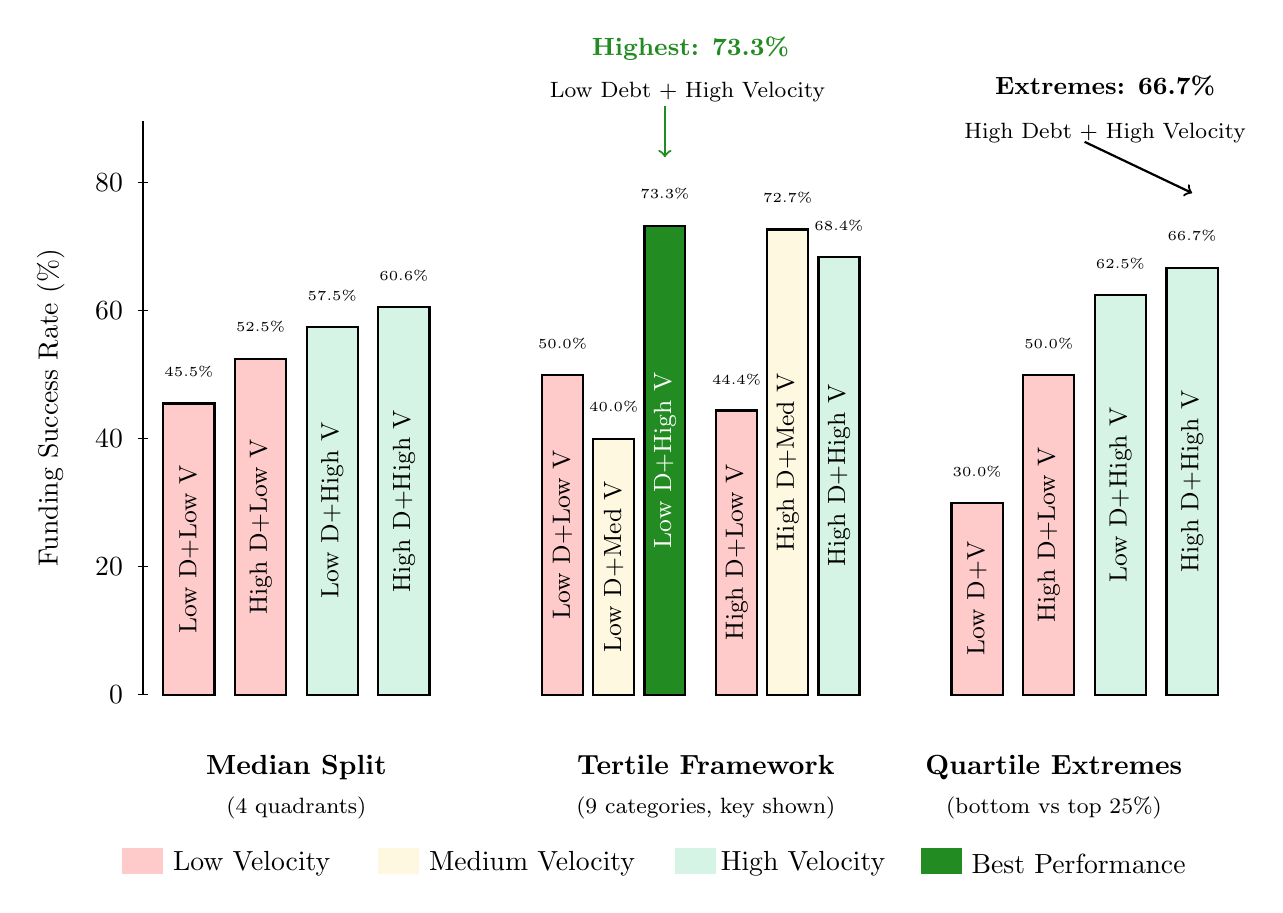
\begin{tikzpicture}[scale=1.3]
    % Define updated subtle colors
    \definecolor{sustainable}{RGB}{213, 244, 230}  % Light green for high velocity
    \definecolor{strategic}{RGB}{255, 248, 225}    % Light yellow for medium velocity  
    \definecolor{premature}{RGB}{219, 234, 254}    % Light blue for mixed/unclear
    \definecolor{burden}{RGB}{254, 202, 202}       % Light red for low velocity
    \definecolor{winner}{RGB}{34, 139, 34}         % Dark green for best performance
    
    % Framework 1: Median Split (4 bars)
    \node[below] at (1.8, -0.5) {\textbf{Median Split}};
    \node[below] at (1.8, -0.9) {\footnotesize (4 quadrants)};
    
    % Low Debt + Low Velocity: 45.5%
    \fill[burden] (0.5, 0) rectangle (1, 2.84375);
    \draw[thick] (0.5, 0) rectangle (1, 2.84375);
    \node[rotate=90, anchor=center, font=\small] at (0.75, 1.42) {Low D+Low V};
    \node[above, font=\tiny] at (0.75, 3.0) {45.5\%};
    
    % High Debt + Low Velocity: 52.5% 
    \fill[burden] (1.2, 0) rectangle (1.7, 3.28125);
    \draw[thick] (1.2, 0) rectangle (1.7, 3.28125);
    \node[rotate=90, anchor=center, font=\small] at (1.45, 1.64) {High D+Low V};
    \node[above, font=\tiny] at (1.45, 3.44) {52.5\%};
    
    % Low Debt + High Velocity: 57.5%
    \fill[sustainable] (1.9, 0) rectangle (2.4, 3.59375);
    \draw[thick] (1.9, 0) rectangle (2.4, 3.59375);
    \node[rotate=90, anchor=center, font=\small] at (2.15, 1.8) {Low D+High V};
    \node[above, font=\tiny] at (2.15, 3.75) {57.5\%};
    
    % High Debt + High Velocity: 60.6%
    \fill[sustainable] (2.6, 0) rectangle (3.1, 3.7875);
    \draw[thick] (2.6, 0) rectangle (3.1, 3.7875);
    \node[rotate=90, anchor=center, font=\small] at (2.85, 1.89) {High D+High V};
    \node[above, font=\tiny] at (2.85, 3.94) {60.6\%};
    
    % Framework 2: Tertile Split (9 bars, showing key ones) - moved left
    \node[below] at (5.8, -0.5) {\textbf{Tertile Framework}};
    \node[below] at (5.8, -0.9) {\footnotesize (9 categories, key shown)};
    
    % Low Debt + Low Velocity: 50.0%
    \fill[burden] (4.2, 0) rectangle (4.6, 3.125);
    \draw[thick] (4.2, 0) rectangle (4.6, 3.125);
    \node[rotate=90, anchor=center, font=\small] at (4.4, 1.56) {Low D+Low V};
    \node[above, font=\tiny] at (4.4, 3.28) {50.0\%};
    
    % Low Debt + Med Velocity: 40.0%
    \fill[strategic] (4.7, 0) rectangle (5.1, 2.5);
    \draw[thick] (4.7, 0) rectangle (5.1, 2.5);
    \node[rotate=90, anchor=center, font=\small] at (4.9, 1.25) {Low D+Med V};
    \node[above, font=\tiny] at (4.9, 2.66) {40.0\%};
    
    % Low Debt + High Velocity: 73.3% (Winner!)
    \fill[winner] (5.2, 0) rectangle (5.6, 4.58125);
    \draw[thick] (5.2, 0) rectangle (5.6, 4.58125);
    \node[rotate=90, anchor=center, font=\small, white] at (5.4, 2.29) {Low D+High V};
    \node[above, font=\tiny] at (5.4, 4.74) {73.3\%};
    
    % High Debt + Low Velocity: 44.4%
    \fill[burden] (5.9, 0) rectangle (6.3, 2.775);
    \draw[thick] (5.9, 0) rectangle (6.3, 2.775);
    \node[rotate=90, anchor=center, font=\small] at (6.1, 1.39) {High D+Low V};
    \node[above, font=\tiny] at (6.1, 2.93) {44.4\%};
    
    % High Debt + Med Velocity: 72.7%
    \fill[strategic] (6.4, 0) rectangle (6.8, 4.54375);
    \draw[thick] (6.4, 0) rectangle (6.8, 4.54375);
    \node[rotate=90, anchor=center, font=\small] at (6.6, 2.27) {High D+Med V};
    \node[above, font=\tiny] at (6.6, 4.7) {72.7\%};
    
    % High Debt + High Velocity: 68.4%
    \fill[sustainable] (6.9, 0) rectangle (7.3, 4.275);
    \draw[thick] (6.9, 0) rectangle (7.3, 4.275);
    \node[rotate=90, anchor=center, font=\small] at (7.1, 2.14) {High D+High V};
    \node[above, font=\tiny] at (7.1, 4.43) {68.4\%};
    
    % Framework 3: Quartile Extremes (4 bars) - moved left
    \node[below] at (9.2, -0.5) {\textbf{Quartile Extremes}};
    \node[below] at (9.2, -0.9) {\footnotesize (bottom vs top 25\%)};
    
    % Very Low Debt + Very Low Velocity: 30.0%
    \fill[burden] (8.2, 0) rectangle (8.7, 1.875);
    \draw[thick] (8.2, 0) rectangle (8.7, 1.875);
    \node[rotate=90, anchor=center, font=\small] at (8.45, 0.94) {Low D+V};
    \node[above, font=\tiny] at (8.45, 2.03) {30.0\%};
    
    % Very High Debt + Very Low Velocity: 50.0%
    \fill[burden] (8.9, 0) rectangle (9.4, 3.125);
    \draw[thick] (8.9, 0) rectangle (9.4, 3.125);
    \node[rotate=90, anchor=center, font=\small] at (9.15, 1.56) {High D+Low V};
    \node[above, font=\tiny] at (9.15, 3.28) {50.0\%};
    
    % Very Low Debt + Very High Velocity: 62.5%
    \fill[sustainable] (9.6, 0) rectangle (10.1, 3.90625);
    \draw[thick] (9.6, 0) rectangle (10.1, 3.90625);
    \node[rotate=90, anchor=center, font=\small] at (9.85, 1.95) {Low D+High V};
    \node[above, font=\tiny] at (9.85, 4.06) {62.5\%};
    
    % Very High Debt + Very High Velocity: 66.7%
    \fill[sustainable] (10.3, 0) rectangle (10.8, 4.16875);
    \draw[thick] (10.3, 0) rectangle (10.8, 4.16875);
    \node[rotate=90, anchor=center, font=\small] at (10.55, 2.08) {High D+High V};
    \node[above, font=\tiny] at (10.55, 4.33) {66.7\%};
    
    % Add Y-axis and labels
    \draw[thick] (0.3, 0) -- (0.3, 5.6);
    \node[rotate=90, anchor=center] at (-0.6, 2.8) {Funding Success Rate (\%)};
    
    \foreach \y/\label in {0/0, 1.25/20, 2.5/40, 3.75/60, 5/80} {
        \draw (0.25, \y) -- (0.35, \y);
        \node[left] at (0.2, \y) {\label};
    }
    
    % Legend
    \fill[burden] (0.1, -1.75) rectangle (0.5, -1.5);
    \node[right] at (0.5, -1.65) {Low Velocity};
    \fill[strategic] (2.6, -1.75) rectangle (3, -1.5);
    \node[right] at (3.0, -1.65) {Medium Velocity};
    \fill[sustainable] (5.5, -1.75) rectangle (5.9, -1.5);
    \node[right] at (5.85, -1.65) {High Velocity};
    \fill[winner] (7.9, -1.75) rectangle (8.3, -1.5);
    \node[right] at (8.3, -1.65) {Best Performance};
    
    % Highlight key findings with better positioned arrows and text
    \draw[thick, ->, color=winner] (5.4, 5.75) -- (5.4, 5.25);
    \node[above, font=\small, color=winner] at (5.65, 6.1) {\textbf{Highest: 73.3\%}};
    \node[above, font=\footnotesize] at (5.62, 5.7) {Low Debt + High Velocity};
    
    \draw[thick, ->] (9.5, 5.4) -- (10.55, 4.9);
    \node[above, font=\small] at (9.7, 5.75) {\textbf{Extremes: 66.7\%}};
    \node[above, font=\footnotesize] at (9.7, 5.3) {High Debt + High Velocity};
    
\end{tikzpicture}
\caption{Cross-Framework Validation: Consistency of Velocity Effect Across Analysis Methods}
\label{fig:sensitivity_comparison}
\end{figure}

\subsection{Performance by Individual Metrics}

To provide additional context for these strategic patterns, we examined funding success across technical debt and velocity quartiles independently. When examining technical debt quartiles (Table~\ref{tab:funding_by_tdr}), the results challenge conventional assumptions by showing that companies in the lowest technical debt quartile achieve the lowest funding success rate (44.4\%). Success rates peak in the second quartile (61.1\%), suggesting that moderate technical debt levels may be optimal rather than minimal debt accumulation. The highest debt quartile maintains strong performance (57.9\%) alongside the highest funding growth rates, indicating that investors do not systematically penalize technical debt when other performance indicators are favorable.

\begin{table}[htbp]
\centering
\caption{Funding Performance by Technical Debt Ratio Quartiles}
\label{tab:funding_by_tdr}
\begin{tabular}{lrrrrr}
\hline
\textbf{TDR Quartile} & \textbf{N} & \textbf{Avg TDR} & \textbf{Success Rate} & \textbf{Funding Growth} & \textbf{Avg Velocity} \\
\hline
Q1 (Lowest Debt) & 36 & 0.006 & 44.4\% & 96.6\% & 0.109 \\
Q2 & 36 & 0.021 & 61.1\% & 194.0\% & 0.139 \\
Q3 & 36 & 0.050 & 52.8\% & 185.1\% & 0.104 \\
Q4 (Highest Debt) & 38 & 0.165 & 57.9\% & 238.4\% & 0.149 \\
\hline
\end{tabular}
\end{table}

In contrast, the analysis of development velocity quartiles (Table~\ref{tab:funding_by_velocity}) reveals a clear monotonic relationship. Funding success rates increase consistently with development velocity, from 47.2\% in the lowest quartile to 68.4\% in the highest quartile, representing a 21.2 percentage point advantage for high-velocity development. This monotonic relationship strongly supports the velocity-focused strategy implications emerging from the quadrant analysis.

\begin{table}[htbp]
\centering
\caption{Funding Performance by Development Velocity Quartiles}
\label{tab:funding_by_velocity}
\begin{tabular}{lrrrrr}
\hline
\textbf{Velocity Quartile} & \textbf{N} & \textbf{Avg Velocity} & \textbf{Success Rate} & \textbf{Funding Growth} & \textbf{Avg TDR} \\
\hline
Q1 (Lowest Velocity) & 36 & 0.029 & 47.2\% & 263.9\% & 0.064 \\
Q2 & 36 & 0.063 & 50.0\% & 160.1\% & 0.047 \\
Q3 & 36 & 0.117 & 50.0\% & 162.7\% & 0.045 \\
Q4 (Highest Velocity) & 38 & 0.285 & 68.4\% & 170.4\% & 0.090 \\
\hline
\end{tabular}
\end{table}

Cross-industry validation demonstrates that these strategic patterns hold consistently across different technical domains, as shown in the sample characteristics analysis. This consistency suggests that the identified relationships reflect fundamental venture capital evaluation dynamics rather than domain-specific phenomena.

\section{Synthesis of Key Findings}\label{sec:results_synthesis}

The empirical analysis yields a coherent set of findings that fundamentally challenge conventional assumptions about technical debt management in startup environments. These results demonstrate that technical debt's strategic impact is context-dependent, with debt accumulation potentially serving as a tool for competitive advantage rather than an unqualified liability when paired with rapid execution capability.

First, technical debt does not systematically constrain development velocity within venture-backed environments (r = 0.056, p = 0.667, company-level). This finding is crucial because it explains why strategic debt accumulation can succeed: debt doesn't automatically slow teams down within typical startup ranges. Technical debt explained only 5.2\% of velocity variance (R² = 0.052), indicating that other factors—team capability, architectural decisions, development infrastructure—dominate execution speed.

Second, the strategic framework analysis establishes that development velocity consistently emerges as the primary success driver across all debt levels. The Strategic Debt quadrant (high debt + high velocity) achieves the highest funding success rate at 60.6\%, while the velocity premium of 8.1-12.0 percentage points remains consistent regardless of debt levels. This pattern holds robustly across multiple analytical frameworks, providing strong evidence for its strategic importance.

The robustness analysis confirms these strategic insights while revealing additional nuances. Moderate technical debt levels may be optimal rather than minimal accumulation, and the velocity advantage remains consistent across different classification schemes and statistical approaches. The finding that companies with the lowest technical debt achieve the lowest funding success rate (44.4\%) particularly challenges traditional engineering wisdom, while the monotonic relationship between velocity and success (47.2\% to 68.4\% across quartiles) reinforces the primacy of execution speed.

These findings provide empirical evidence for a context-dependent view of technical debt management that acknowledges the unique incentive structures and competitive pressures of venture-backed environments. During periods of capital abundance such as the \ac{ZIRP} era, the market appears to reward demonstrated execution velocity over internal code quality metrics, supporting strategic frameworks where technical debt accumulation serves as "temporal arbitrage"—trading future development capacity for immediate competitive advantage when current execution capability is more valuable than equivalent future capacity. This represents a fundamental departure from traditional software engineering approaches that universally characterize technical debt as a liability to be minimized, suggesting instead that optimal strategies depend critically on macroeconomic conditions, competitive dynamics, and organizational objectives.